\section{Task 2 \\ Benchmarking move sorting}
\color{gray}
\textit{The following tests where executed on an ubuntu distrubution run in an VM with 2 Gb of DDR4 RAM and an i7-6700HQ skylake processor.}\\\\
\color{black}
In the following analyse we do concentrate on the amount of nodes generated by the search tree and the time it took the compute a move. The other benchmarks we implement were, as expected, not affected by move sorting in a notable way.\\\\
Except the first map, every map is analysed in 3 different states. The first one being the initial state, the second one in the middle of a game (at least 30\% of stones placed). The last possible state is and end game state where 90\% of the cells are occupied.\\
The maps taken for the benchmark partially taken from the server logs and partially created by us.\\
The results are discussed at the end and not after every map as the results should be similar for the most parts.\\
\newpage
\textbf{A list of the maps used for the tests:}\\\\
\begin{figure}[!hp]
	\centering
	\includegraphics[width=0.6\textwidth,keepaspectratio]{FunnelOfDeath.png}\\
	\caption{FunnelOfDeath}
\end{figure}

\begin{figure}[H]
	\centering
	\includegraphics[width=0.6\textwidth,keepaspectratio]{g3_2}\\
	\caption{g3\_2}
\end{figure}

\begin{figure}[H]
	\centering
	\includegraphics[width=0.6\textwidth,keepaspectratio]{reversi.png}\\
	\caption{Standart}
\end{figure}

\begin{figure}[H]
	\centering
	\includegraphics[width=0.6\textwidth,keepaspectratio]{TripleOfTraps.png}\\
	\caption{TripleOfTraps}
\end{figure}

\begin{figure}[H]
	\centering
	\includegraphics[width=0.6\textwidth,keepaspectratio]{g5_1.png}\\
	\caption{g5\_1}
\end{figure}

\newpage
\textbf{Map: }Funnel of Death\\

\textbf{State: }Start\\

\textbf{Results: }\\\\

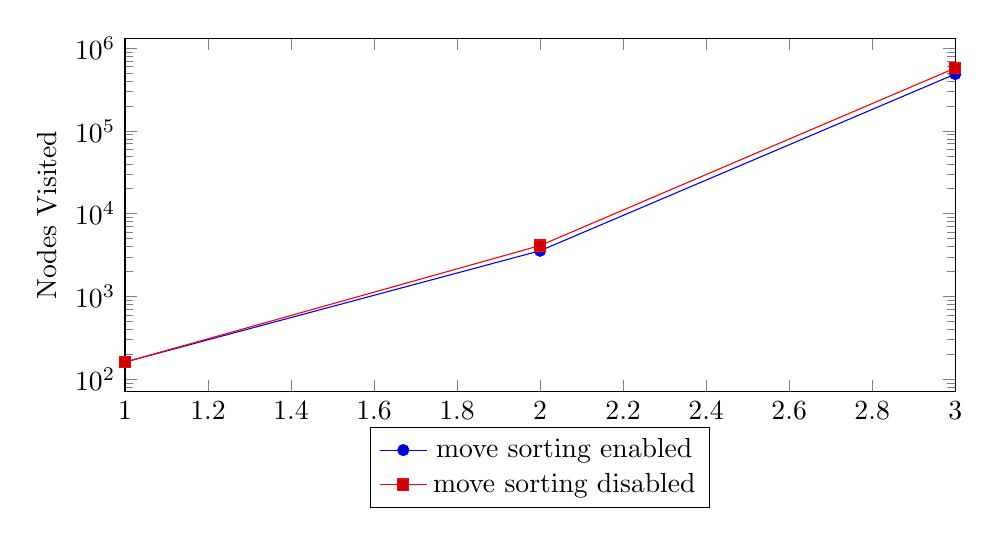
\begin{tikzpicture}
\begin{axis}[
height=0.5\textwidth,
width=\textwidth,
xlabel=Depth,
xmin=1,
xmax=3,
ylabel=Nodes Visited,
ymin=0,
ymode=log,
legend style={at={(0.5,-0.1)},anchor=north}
]
\addplot table {
	1 161
	2 3564
	3 486203
};
\addlegendentry{move sorting enabled}
\addplot table {
	1 161
	2 4121
	3 574940
};
\addlegendentry{move sorting disabled}
\end{axis}
\end{tikzpicture}\\\\

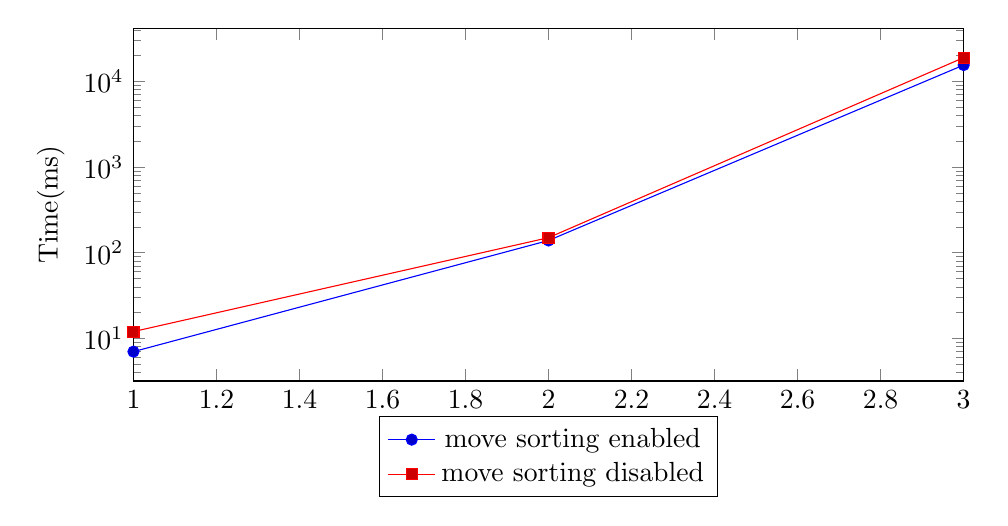
\begin{tikzpicture}
\begin{axis}[
height=0.5\textwidth,
width=\textwidth,
xlabel=Depth,
xmin=1,
xmax=3,
ylabel=Time(ms),
ymin=0,
ymode=log,
legend style={at={(0.5,-0.1)},anchor=north}
]
\addplot table {
	1 7
	2 139
	3 15540
};
\addlegendentry{move sorting enabled}
\addplot table {
	1 12
	2 150
	3 18977
};
\addlegendentry{move sorting disabled}
\end{axis}
\end{tikzpicture}
\newpage

\textbf{Map: }g3\_2\\

\textbf{State: }Start\\

\textbf{Results: }\\\\

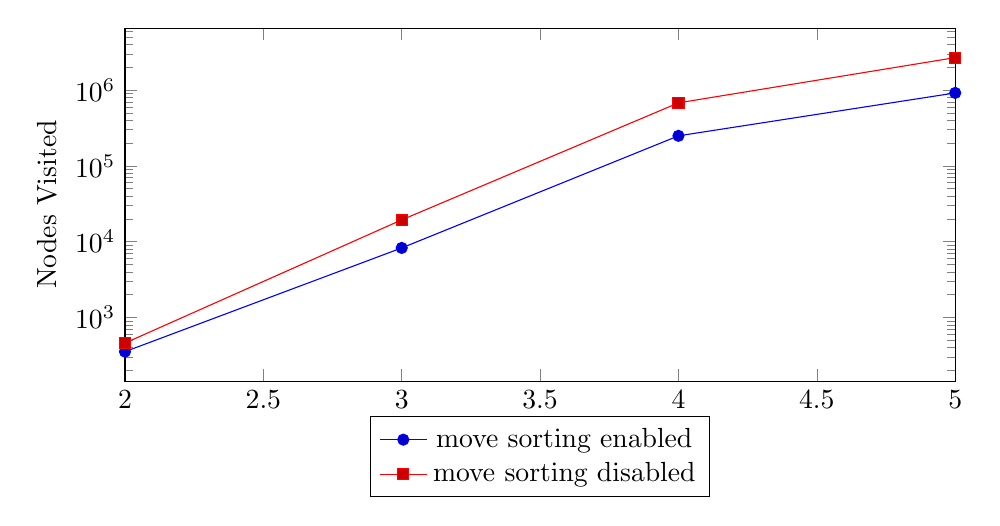
\begin{tikzpicture}
\begin{axis}[
height=0.5\textwidth,
width=\textwidth,
xlabel=Depth,
xmin=2,
xmax=5,
ylabel=Nodes Visited,
ymin=0,
ymode=log,
legend style={at={(0.5,-0.1)},anchor=north}
]
\addplot table {
	2 355
	3 8280
	4 248977
	5 915754
};
\addlegendentry{move sorting enabled}
\addplot table {
	2 461
	3 19408
	4 677463
	5 2675505
};
\addlegendentry{move sorting disabled}
\end{axis}
\end{tikzpicture}\\\\

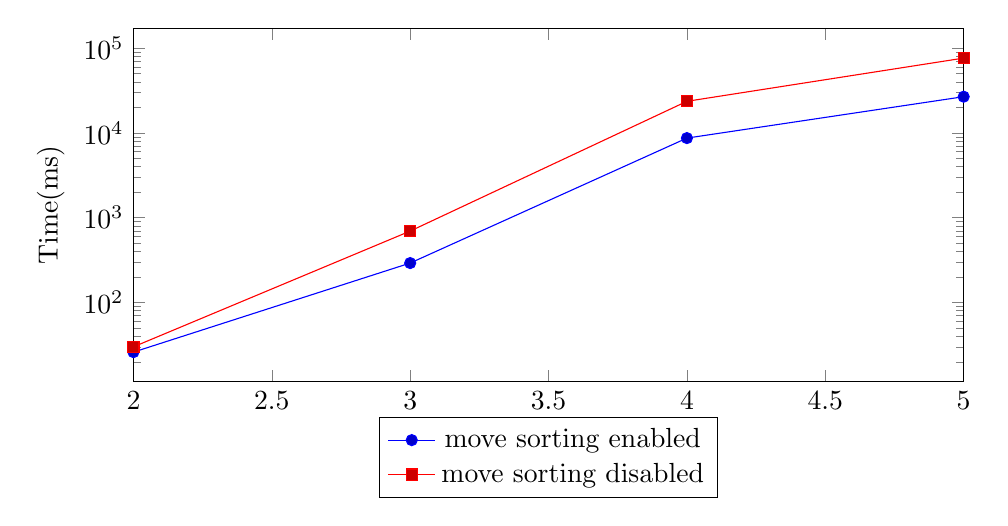
\begin{tikzpicture}
\begin{axis}[
height=0.5\textwidth,
width=\textwidth,
xlabel=Depth,
xmin=2,
xmax=5,
ylabel=Time(ms),
ymin=0,
ymode=log,
legend style={at={(0.5,-0.1)},anchor=north}
]
\addplot table {
	2 26
	3 292
	4 8694
	5 26764
};
\addlegendentry{move sorting enabled}
\addplot table {
	2 30
	3 696
	4 23614
	5 76348
};
\addlegendentry{move sorting disabled}
\end{axis}
\end{tikzpicture}
\newpage

\textbf{Map: }g3\_2\\

\textbf{State: }End\\

\textbf{Results: }\\\\

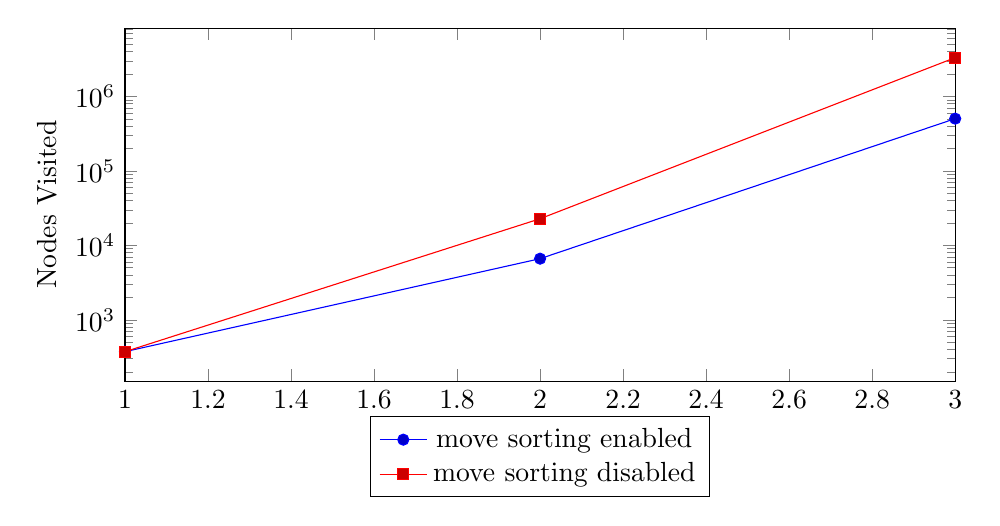
\begin{tikzpicture}
\begin{axis}[
height=0.5\textwidth,
width=\textwidth,
xlabel=Depth,
xmin=1,
xmax=3,
ylabel=Nodes Visited,
ymin=0,
ymode=log,
legend style={at={(0.5,-0.1)},anchor=north}
]
\addplot table {
	1 373
	2 6625
	3 504311
};
\addlegendentry{move sorting enabled}
\addplot table {
	1 373
	2 22793
	3 3331443
};
\addlegendentry{move sorting disabled}
\end{axis}
\end{tikzpicture}\\\\

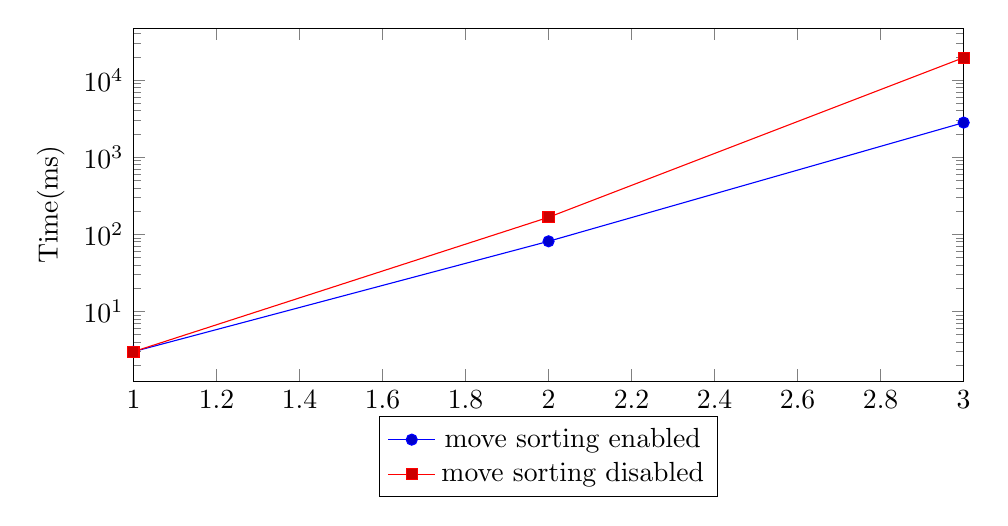
\begin{tikzpicture}
\begin{axis}[
height=0.5\textwidth,
width=\textwidth,
xlabel=Depth,
xmin=1,
xmax=3,
ylabel=Time(ms),
ymin=0,
ymode=log,
legend style={at={(0.5,-0.1)},anchor=north}
]
\addplot table {
	1 3
	2 81
	3 2807
};
\addlegendentry{move sorting enabled}
\addplot table {
	1 3
	2 166
	3 19549
};
\addlegendentry{move sorting disabled}
\end{axis}
\end{tikzpicture}
\newpage

\textbf{Map: }Standard\\

\textbf{State: }Start\\

\textbf{Results: }\\\\

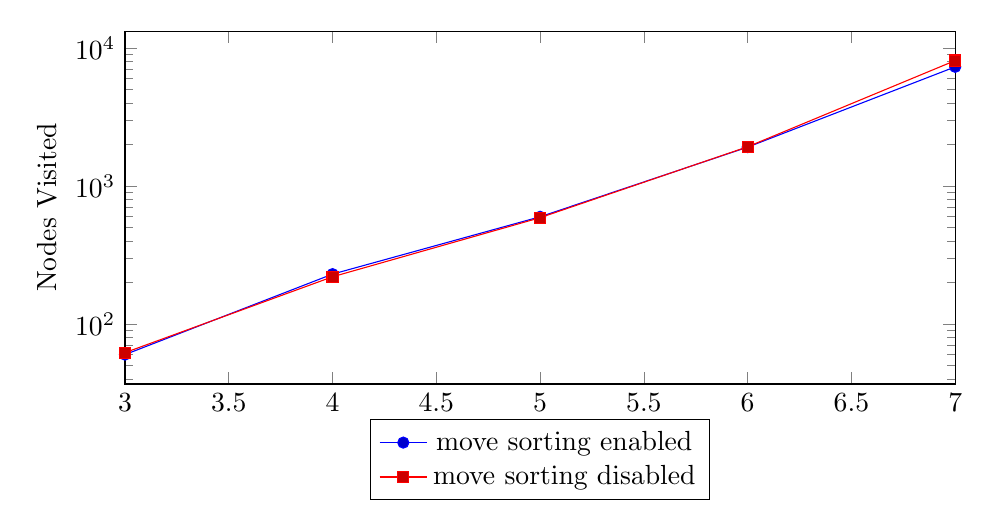
\begin{tikzpicture}
\begin{axis}[
height=0.5\textwidth,
width=\textwidth,
xlabel=Depth,
xmin=3,
xmax=7,
ylabel=Nodes Visited,
ymin=0,
ymode=log,
legend style={at={(0.5,-0.1)},anchor=north}
]
\addplot table {
	3 60
	4 230
	5 599
	6 1916
	7 7319
	8 28118
	9 89217
	10 360392
};
\addlegendentry{move sorting enabled}
\addplot table {
	3 62
	4 220
	5 590
	6 1928
	7 8129
	8 29054
	9 96813
	10 395322	
};
\addlegendentry{move sorting disabled}
\end{axis}
\end{tikzpicture}\\\\

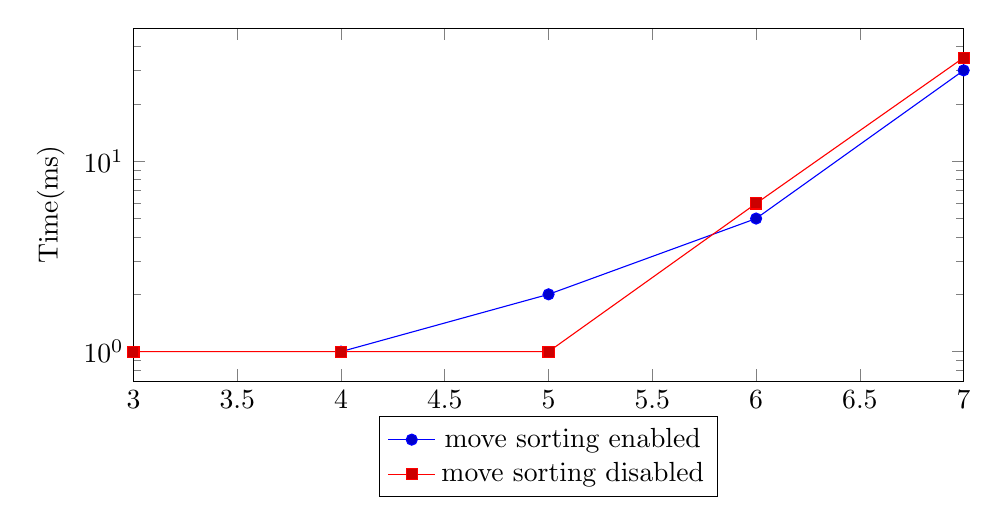
\begin{tikzpicture}
\begin{axis}[
height=0.5\textwidth,
width=\textwidth,
xlabel=Depth,
xmin=3,
xmax=7,
ylabel=Time(ms),
ymin=0,
ymode=log,
legend style={at={(0.5,-0.1)},anchor=north}
]
\addplot table {
	3 0
	4 1
	5 2
	6 5
	7 30
	8 115
	9 227
	10 926
};
\addlegendentry{move sorting enabled}
\addplot table {
	3 1
	4 1
	5 1
	6 6
	7 35
	8 158
	9 289
	10 1001
};
\addlegendentry{move sorting disabled}
\end{axis}
\end{tikzpicture}
\newpage

\textbf{Map: }Standard\\

\textbf{State: }Mid\\

\textbf{Results: }\\\\

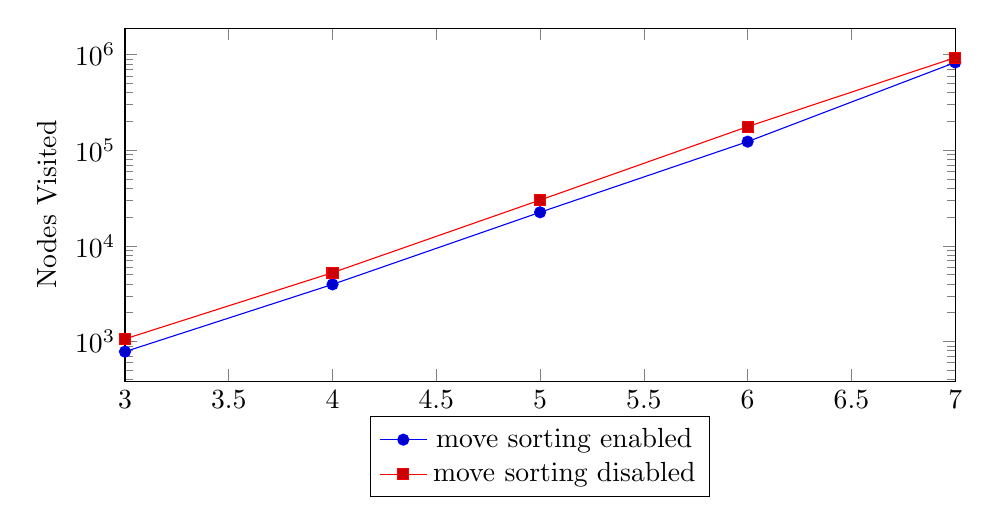
\begin{tikzpicture}
\begin{axis}[
height=0.5\textwidth,
width=\textwidth,
xlabel=Depth,
xmin=3,
xmax=7,
ylabel=Nodes Visited,
ymin=0,
ymode=log,
legend style={at={(0.5,-0.1)},anchor=north}
]
\addplot table {
	3 782
	4 3952
	5 22443
	6 122989
	7 828357
	
};
\addlegendentry{move sorting enabled}
\addplot table {
	3 1063
	4 5241
	5 30138
	6 176629
	7 930299
};
\addlegendentry{move sorting disabled}
\end{axis}
\end{tikzpicture}\\\\

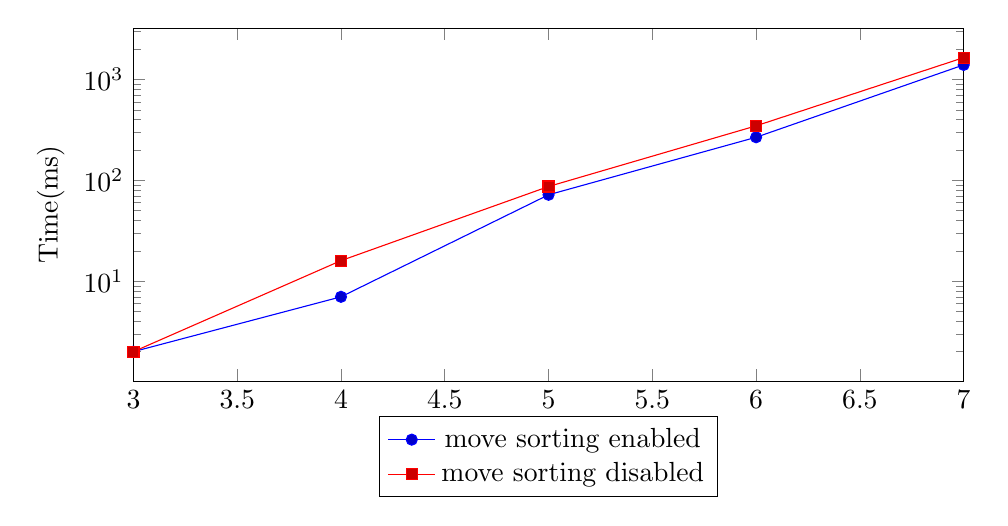
\begin{tikzpicture}
\begin{axis}[
height=0.5\textwidth,
width=\textwidth,
xlabel=Depth,
xmin=3,
xmax=7,
ylabel=Time(ms),
ymin=0,
ymode=log,
legend style={at={(0.5,-0.1)},anchor=north}
]
\addplot table {
	3 2
	4 7
	5 72
	6 268
	7 1400
};
\addlegendentry{move sorting enabled}
\addplot table {
	3 2
	4 16
	5 87
	6 348
	7 1653
};
\addlegendentry{move sorting disabled}
\end{axis}
\end{tikzpicture}
\newpage

\textbf{Map: }Standard\\

\textbf{State: }End\\

\textbf{Results: }\\\\

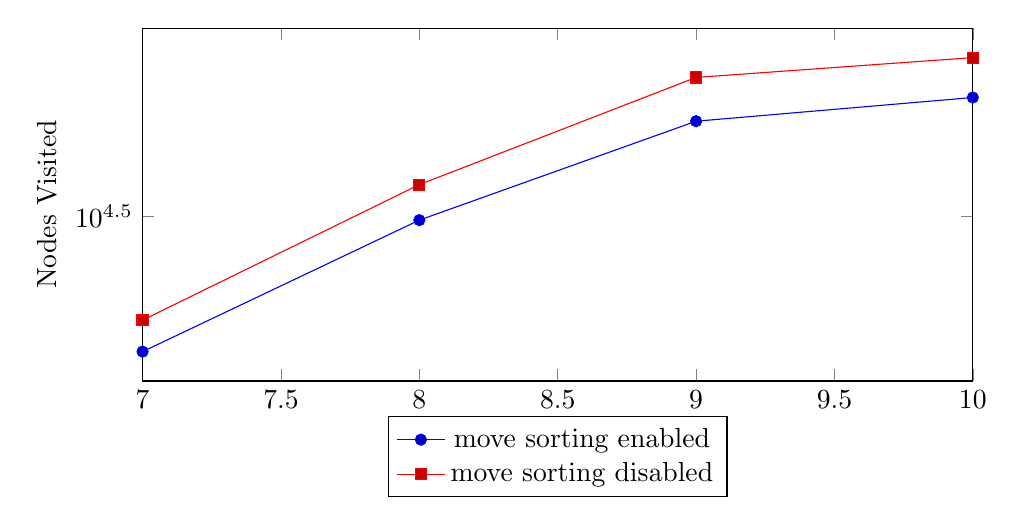
\begin{tikzpicture}
\begin{axis}[
height=0.5\textwidth,
width=\textwidth,
xlabel=Depth,
xmin=7,
xmax=10,
ylabel=Nodes Visited,
ymin=0,
ymode=log,
legend style={at={(0.5,-0.1)},anchor=north}
]
\addplot table {
	7 15736
	8 31044
	9 51752
	10 58493
};
\addlegendentry{move sorting enabled}
\addplot table {
	7 18517
	8 37292
	9 64890
	10 71882
};
\addlegendentry{move sorting disabled}
\end{axis}
\end{tikzpicture}\\\\

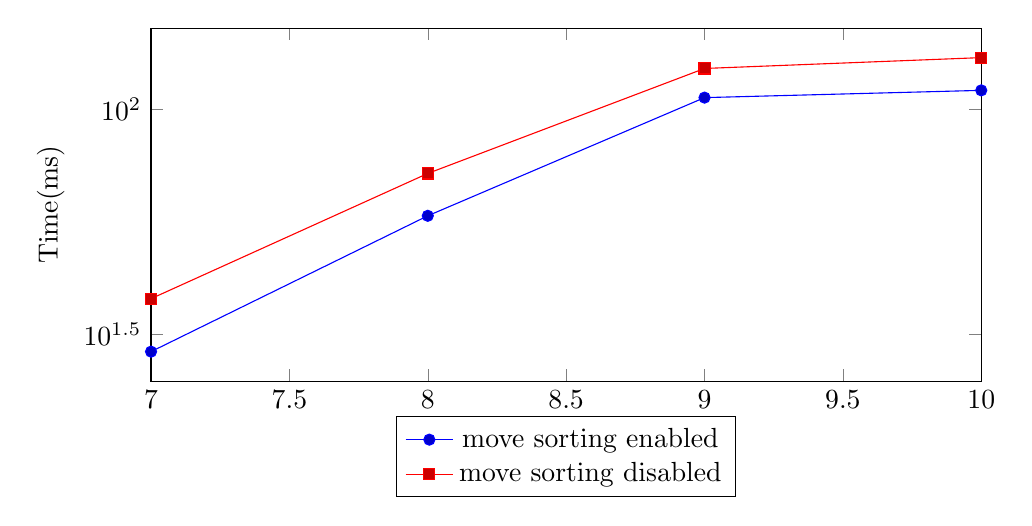
\begin{tikzpicture}
\begin{axis}[
height=0.5\textwidth,
width=\textwidth,
xlabel=Depth,
xmin=7,
xmax=10,
ylabel=Time(ms),
ymin=0,
ymode=log,
legend style={at={(0.5,-0.1)},anchor=north}
]
\addplot table {
	7 29
	8 58
	9 106
	10 110
};
\addlegendentry{move sorting enabled}
\addplot table {
	7 38
	8 72
	9 123
	10 130
};
\addlegendentry{move sorting disabled}
\end{axis}
\end{tikzpicture}
\newpage

\textbf{Map: }TripleOfTraps\\

\textbf{State: }Start\\

\textbf{Results: }\\\\

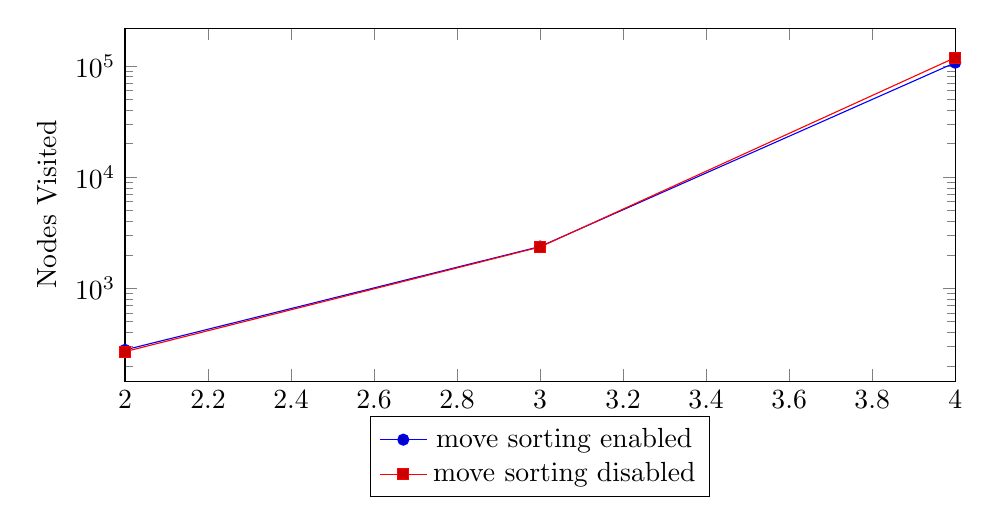
\begin{tikzpicture}
\begin{axis}[
height=0.5\textwidth,
width=\textwidth,
xlabel=Depth,
xmin=2,
xmax=4,
ylabel=Nodes Visited,
ymin=0,
ymode=log,
legend style={at={(0.5,-0.1)},anchor=north}
]
\addplot table {
	2 279
	3 2373
	4 106888
};
\addlegendentry{move sorting enabled}
\addplot table {
	2 269
	3 2352
	4 118688
};
\addlegendentry{move sorting disabled}
\end{axis}
\end{tikzpicture}\\\\

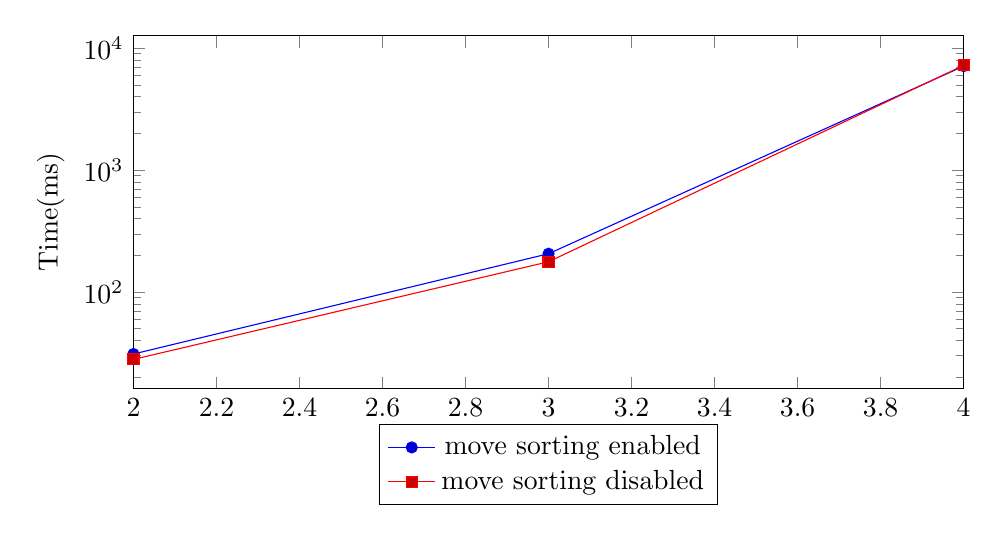
\begin{tikzpicture}
\begin{axis}[
height=0.5\textwidth,
width=\textwidth,
xlabel=Depth,
xmin=2,
xmax=4,
ylabel=Time(ms),
ymin=0,
ymode=log,
legend style={at={(0.5,-0.1)},anchor=north}
]
\addplot table {
	2 31
	3 206
	4 7120
};
\addlegendentry{move sorting enabled}
\addplot table {
	2 28
	3 177
	4 7228
};
\addlegendentry{move sorting disabled}
\end{axis}
\end{tikzpicture}
\newpage

\textbf{Map: }TripleOfTraps\\

\textbf{State: }Mid\\

\textbf{Results: }\\\\

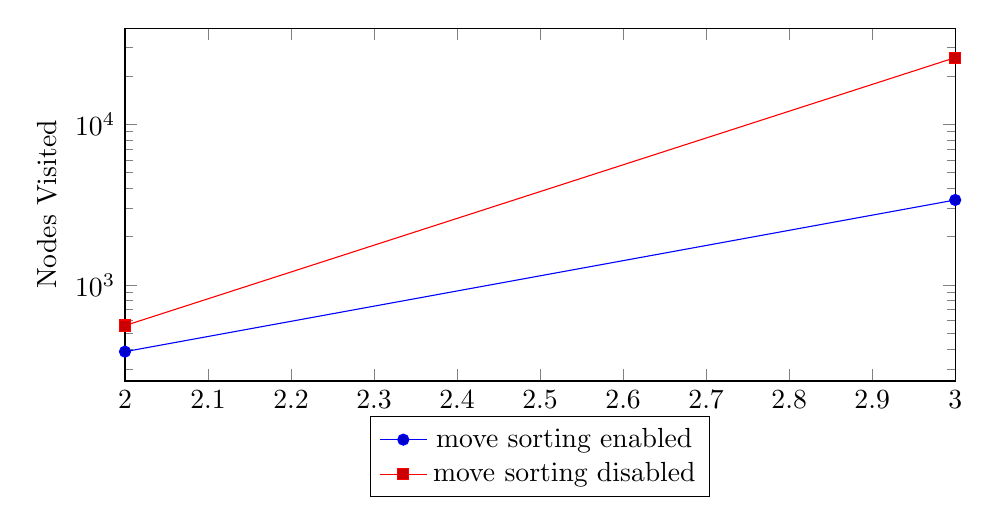
\begin{tikzpicture}
\begin{axis}[
height=0.5\textwidth,
width=\textwidth,
xlabel=Depth,
xmin=2,
xmax=3,
ylabel=Nodes Visited,
ymin=0,
ymode=log,
legend style={at={(0.5,-0.1)},anchor=north}
]
\addplot table {
	2 384
	3 3380
};
\addlegendentry{move sorting enabled}
\addplot table {
	2 558
	3 26042
};
\addlegendentry{move sorting disabled}
\end{axis}
\end{tikzpicture}\\\\

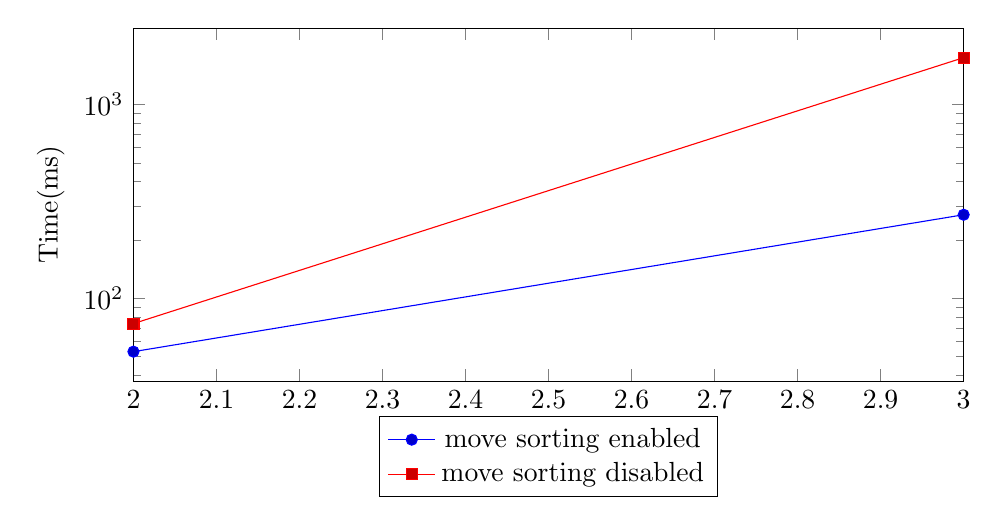
\begin{tikzpicture}
\begin{axis}[
height=0.5\textwidth,
width=\textwidth,
xlabel=Depth,
xmin=2,
xmax=3,
ylabel=Time(ms),
ymin=0,
ymode=log,
legend style={at={(0.5,-0.1)},anchor=north}
]
\addplot table {
	2 53
	3 270
};
\addlegendentry{move sorting enabled}
\addplot table {
	2 74
	3 1749
};
\addlegendentry{move sorting disabled}
\end{axis}
\end{tikzpicture}
\newpage

\textbf{Map: }g5\_1\\

\textbf{State: }Start\\

\textbf{Results: }\\\\

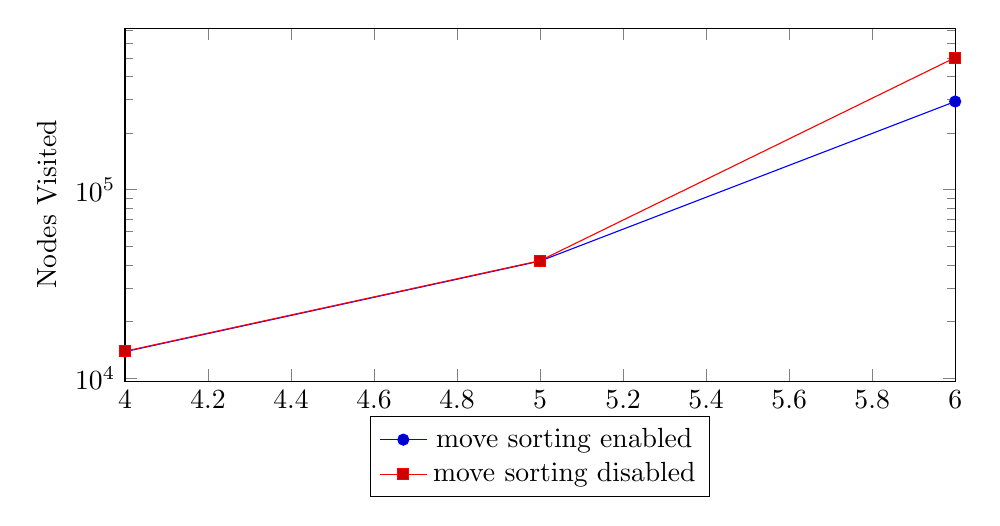
\begin{tikzpicture}
\begin{axis}[
height=0.5\textwidth,
width=\textwidth,
xlabel=Depth,
xmin=4,
xmax=6,
ylabel=Nodes Visited,
ymin=0,
ymode=log,
legend style={at={(0.5,-0.1)},anchor=north}
]
\addplot table {
	4 13846
	5 41852
	6 293762
};
\addlegendentry{move sorting enabled}
\addplot table {
	4 13920
	5 42061
	6 502012
};
\addlegendentry{move sorting disabled}
\end{axis}
\end{tikzpicture}\\\\

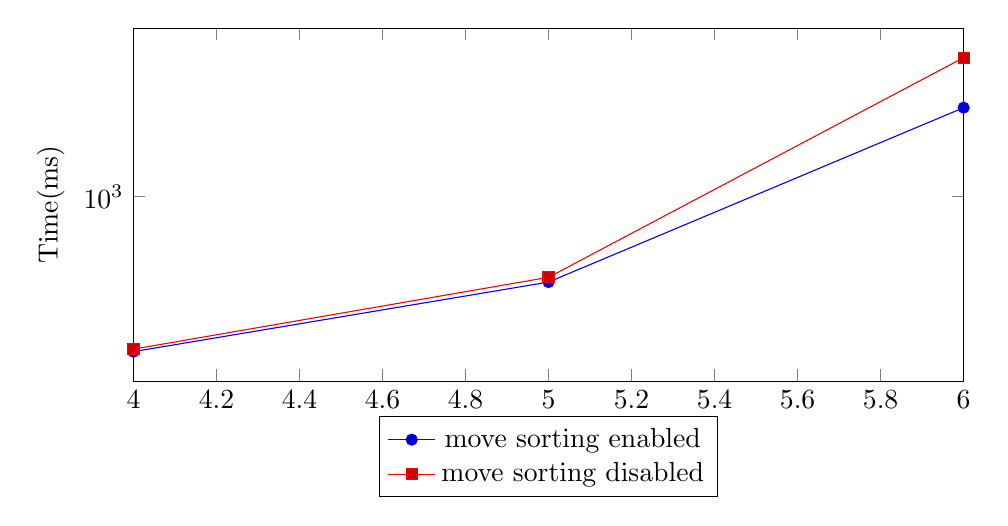
\begin{tikzpicture}
\begin{axis}[
height=0.5\textwidth,
width=\textwidth,
xlabel=Depth,
xmin=4,
xmax=6,
ylabel=Time(ms),
ymin=0,
ymode=log,
legend style={at={(0.5,-0.1)},anchor=north}
]
\addplot table {
	4 175
	5 383
	6 2725
};
\addlegendentry{move sorting enabled}
\addplot table {
	4 180
	5 404
	6 4786
};
\addlegendentry{move sorting disabled}
\end{axis}
\end{tikzpicture}
\newpage
\textbf{Map: }g5\_1\\

\textbf{State: }End\\

\textbf{Results: }\\\\

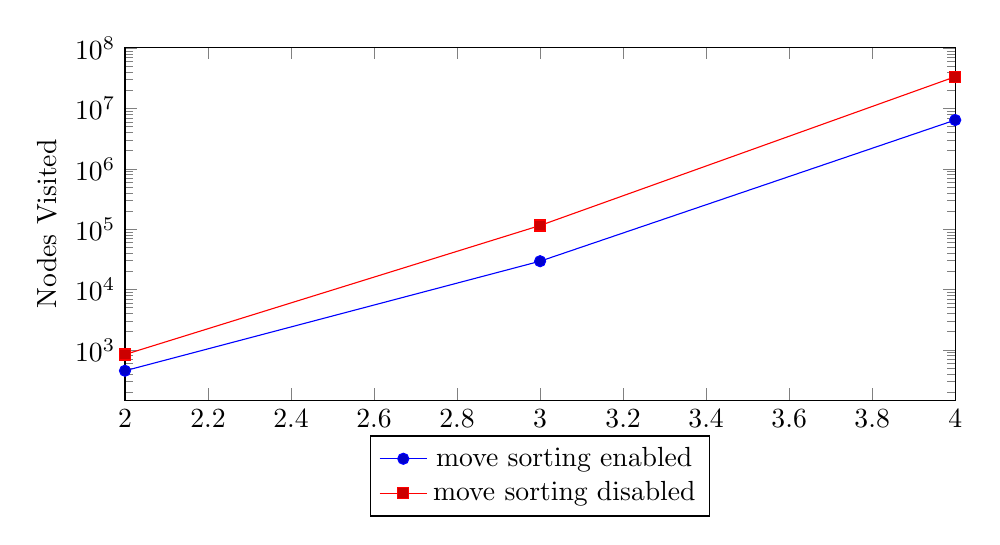
\begin{tikzpicture}
\begin{axis}[
height=0.5\textwidth,
width=\textwidth,
xlabel=Depth,
xmin=2,
xmax=4,
ylabel=Nodes Visited,
ymin=0,
ymode=log,
legend style={at={(0.5,-0.1)},anchor=north}
]
\addplot table {
	2 449
	3 29396
	4 6434422
};
\addlegendentry{move sorting enabled}
\addplot table {
	2 835
	3 114886
	4 33609315
};
\addlegendentry{move sorting disabled}
\end{axis}
\end{tikzpicture}\\\\

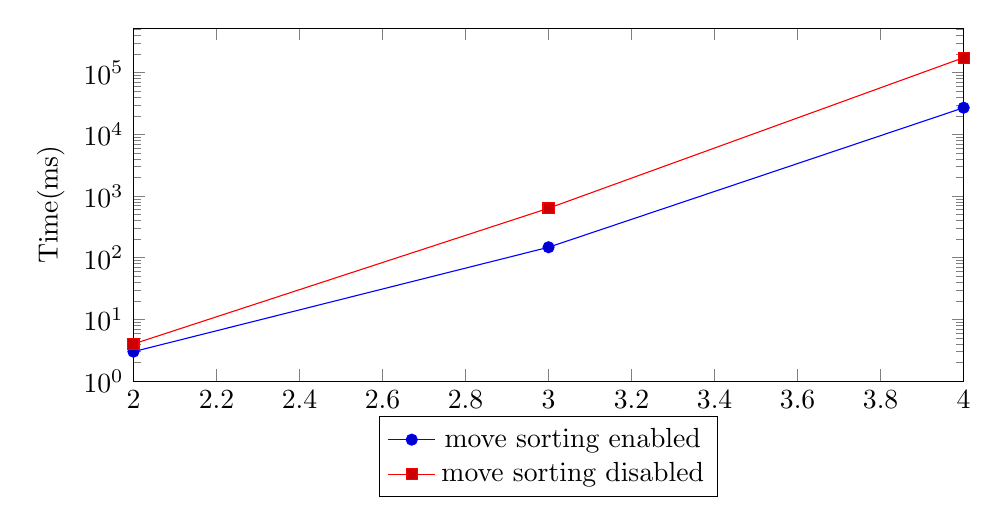
\begin{tikzpicture}
\begin{axis}[
height=0.5\textwidth,
width=\textwidth,
xlabel=Depth,
xmin=2,
xmax=4,
ylabel=Time(ms),
ymin=0,
ymode=log,
legend style={at={(0.5,-0.1)},anchor=north}
]
\addplot table {
	2 3
	3 148
	4 27083
};
\addlegendentry{move sorting enabled}
\addplot table {
	2 4
	3 635
	4 175808
};
\addlegendentry{move sorting disabled}
\end{axis}
\end{tikzpicture}
\newpage

{\Large \textbf{Analyse}}\\\\
Enabling move sorting is for almost every case more efficient. Overall move sorting seems to be nearly equal to normal alpha beta pruning at low depth and faster at higher depth. The difference is noticeable but not extraordinary.\\
Exceptions are:\\
\begin{itemize}
	\item At depth 1 move sorting is slower. This has to do with the overhead of managing the lists.
	\item States at which nearly all cells are occupied \textit{(Standard(end state))}. Here alpha beta pruning without move sorting is faster. This lets use suppose that move sorting is only useful if the game tree is in fact growing exponentially.
	\item \textit{(TripleOfTraps(mid state))} In this case move sorting is over an order of magnitude faster. This might have to with an lucky order of moves.
	\item \textit{(Standart(start state))} During this evaluation we found that move sorting is fast for depth 6 and 7. This seems strange but can have to do with us only using a pseudo sorted list and an unlucky order of moves.
\end{itemize}


